\documentclass[12pt]{article}
\usepackage[utf8]{inputenc}
\usepackage{geometry}
\geometry{legalpaper, margin=1in, top=10mm}
\usepackage{graphicx}
\usepackage{caption}
\usepackage[export]{adjustbox}
\usepackage{mathptmx}
\usepackage{secdot}
\usepackage{amsmath}
\usepackage{mwe}
\usepackage{subfig}
\usepackage[framed,numbered,autolinebreaks,useliterate]{mcode}
\usepackage{xcolor}
\usepackage{listings}

\definecolor{mGreen}{rgb}{0,0.6,0}
\definecolor{mGray}{rgb}{0.5,0.5,0.5}
\definecolor{mPurple}{rgb}{0.58,0,0.82}
\definecolor{backgroundColour}{rgb}{0.95,0.95,0.92}

\usepackage{hyperref}
\newcommand\Tstrut{\rule{0pt}{2.6ex}}         % = `top' strut
\newcommand\Bstrut{\rule[-0.9ex]{0pt}{0pt}}   % = `bottom' strut
\AtBeginDocument{\hypersetup{pdfborder={0 0 1}}}
\lstdefinestyle{CStyle}{
	backgroundcolor=\color{white},   
	commentstyle=\color{mGreen},
	keywordstyle=\color{magenta},
	numberstyle=\tiny\color{mGray},
	stringstyle=\color{mPurple},
	basicstyle=\footnotesize,
	breakatwhitespace=false,         
	breaklines=true,                 
	captionpos=b,                    
	keepspaces=true,                 
	numbers=left,                    
	numbersep=5pt,                  
	showspaces=false,                
	showstringspaces=false,
	showtabs=false,                  
	tabsize=2,
	language=C
}
\title{%
	Dynamics and Control \\
	\large Homework 2 }

\author{Jinaykumar Patel \\ 1001937580}

\date{}
\begin{document}
	\maketitle
	
\section{System Identification}
Given that the system dynamics is of form 
\begin{equation}
	\tau=I \ddot{\Theta}+B \dot{\Theta}+G(\Theta)
\end{equation}
Inertia of the arm $(I)$, the viscous friction in the joint $(B)$ and by gravity $(G)$.\\
It is given that the function \textit{PD\_control()} receives all relevant information from the robot system and is called at a rate of $500 \; Hz$, i.e. $\mathbf{0.002 \; sec}$.\\

In order to identity the system parameters ($I, B, G$), first the gravity and viscous friction term should be identified. Few experiments are done to predict the gravity term by returning random numbers from the function \textit{PD\_Control()}. 
Also, the form gravity term could be easily determine from the force analysis. The gravity force always act downwards. Assuming the mass of robot manipulator to be $m$ and length $l$, taking the components of this force we can seen from fig. (\ref{fig1}) that the component $mg \cos{\theta}$ is responsible for the torque and it is perpendicular to the position vector. The other component  $mg \sin{\theta}$ acts along the direction of position vector (or the length) hence, it doesn't produce any torque. Hence, the torque due to gravity is therefore $\mathbf{l \times mg \cos{\theta}}$ or $\mathbf{mgl\cos{\theta}}$. Following is the code for the gravity term identification, where the constant number in the term is identified to be equal to \framebox[1.1\width]{$\mathbf{2.205195}$}.

\begin{lstlisting}[style=CStyle]
	#include <stdio.h>
	#include <math.h>
	#include <stdlib.h>
	#ifndef M_PI
	#define M_PI 3.1415927
	#endif
	
	int UTA_ID = 1001937580;
	
	
	double PD_control(theta, theta_dot, theta_ref, theta_dot_ref)
	double theta, theta_dot, theta_ref, theta_dot_ref;
	{
		
		printf("%f %f\n", theta, theta_dot);
		return (2.205195*cos(theta));
	}
\end{lstlisting}

\begin{figure}[h]
	\centering{\includegraphics[trim={2cm 6cm 2cm 4cm},clip,width=0.4\columnwidth]{Part1.pdf}}
	\vspace{-1mm}
	\caption{Gravity force acting through center of gravity}
	\label{fig1}
\end{figure}

Now that we have $G(\Theta)$, we can compensate for it and look for a way to get $\ddot{\mathbf{\theta}} = 0$. Need to achieve constant velocity, hence apply a constant torque and gravity compensation, i.e. 
\begin{equation}
	\tau +G(\theta)=I \ddot{\theta}+B \dot{\theta}+G(\theta)
\end{equation}
System will eventually reach constant velocity, i.e. $\ddot{\theta}=0$ 
\begin{equation}\label{eq:3}
	\tau=B \dot{\theta} \quad \Rightarrow \quad B=\frac{\tau}{\dot{\theta}}
\end{equation}
Three experiments are performed while applying different constant torques of $(1, 2, 5)$ units. Fig. (\ref{fig2}) shows these different experiments which shows that it reach a constant value of $\dot{\theta}$. From eq. (\ref{eq:3}) we can arrive with the value of $B$. Following is the code snippet for this case, where $B$ turns out to be equal to \framebox[1.1\width]{$\mathbf{0.815009}$}.
\begin{lstlisting}[style=CStyle]
	#include <stdio.h>
	#include <math.h>
	#include <stdlib.h>
	#ifndef M_PI
	#define M_PI 3.1415927
	#endif
	
	int UTA_ID = 1001937580;
	
	
	double PD_control(theta, theta_dot, theta_ref, theta_dot_ref)
	double theta, theta_dot, theta_ref, theta_dot_ref;
	{
		
		double tau = 1; // tau = 2; // tau = 5;
		//double B = 0.815009;
		//double B = tau/theta_dot;
		//printf("%f\n", theta_dot); //B = 0.815009;
		
		printf("%f %f\n", theta, theta_dot);
		return (tau + 2.205195*cos(theta));
	}
\end{lstlisting}	

\begin{figure}
	
	\begin{minipage}{.5\linewidth}
		\centering
		\subfloat[]{\label{main:a}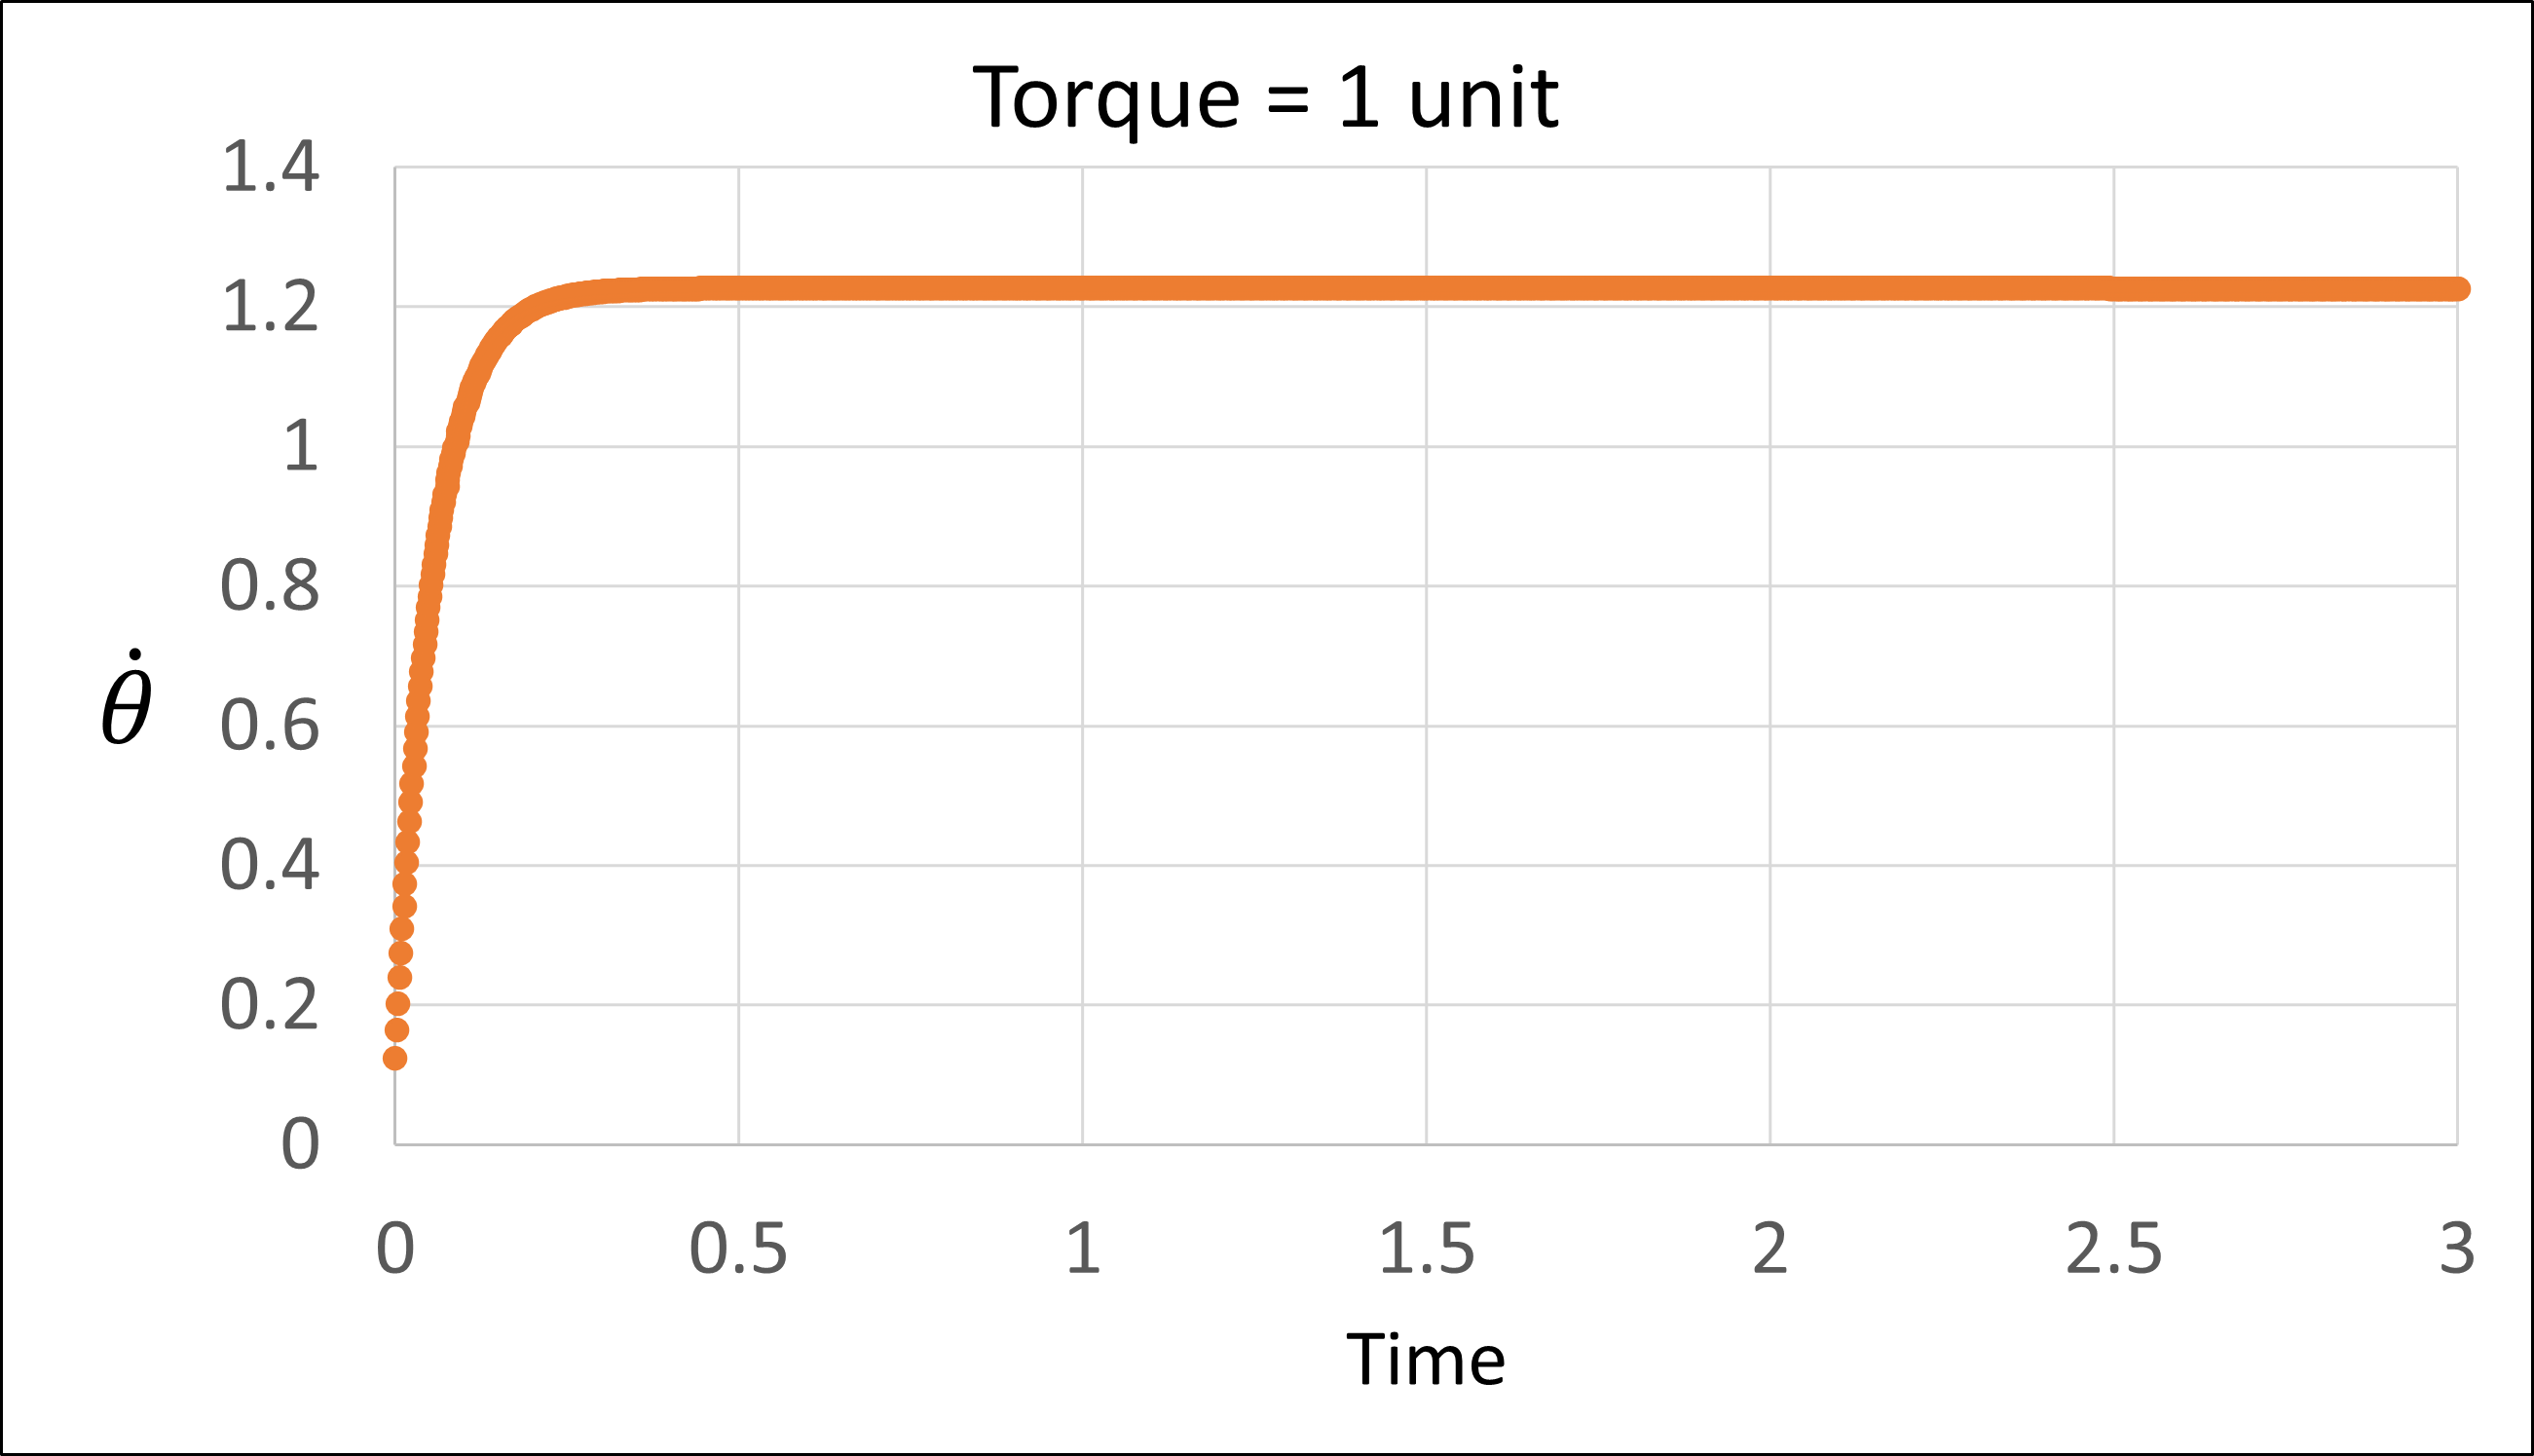
\includegraphics[scale=.4]{Picture1.png}}
	\end{minipage}%
	\begin{minipage}{.5\linewidth}
		\centering
		\subfloat[]{\label{main:b}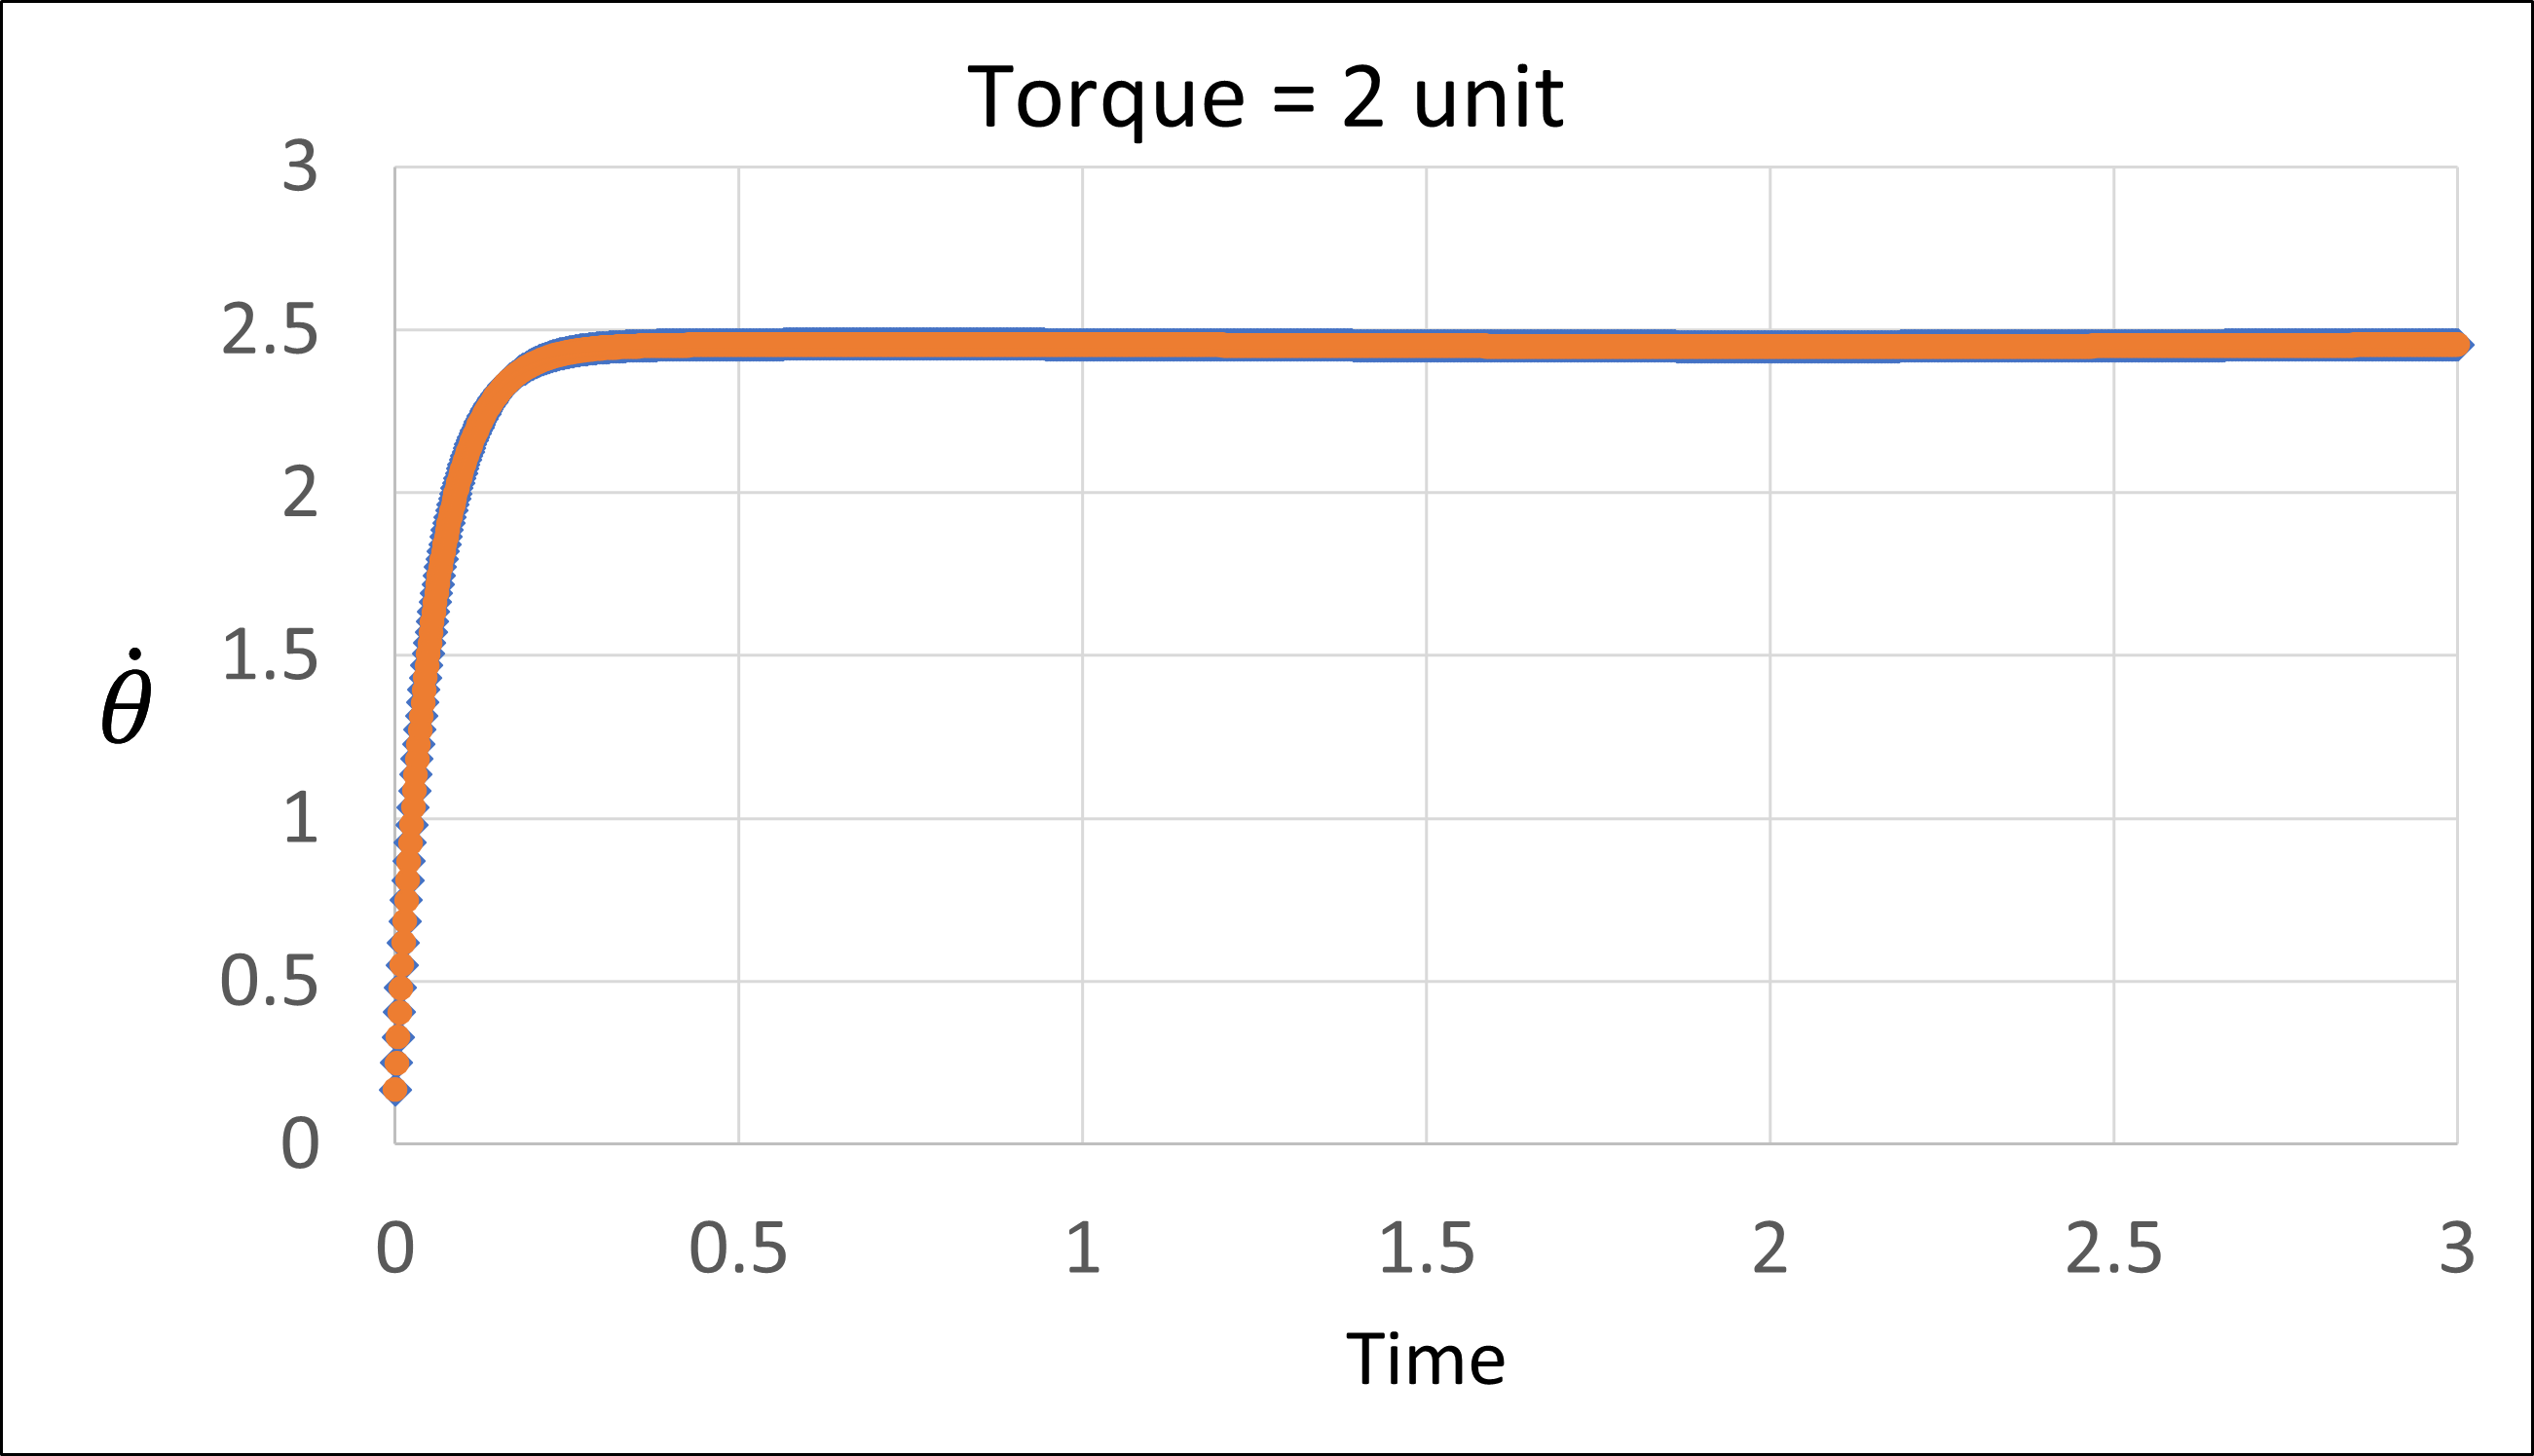
\includegraphics[scale=.4]{Picture2.png}}
	\end{minipage}\par\medskip
	\centering
	\subfloat[]{\label{main:c}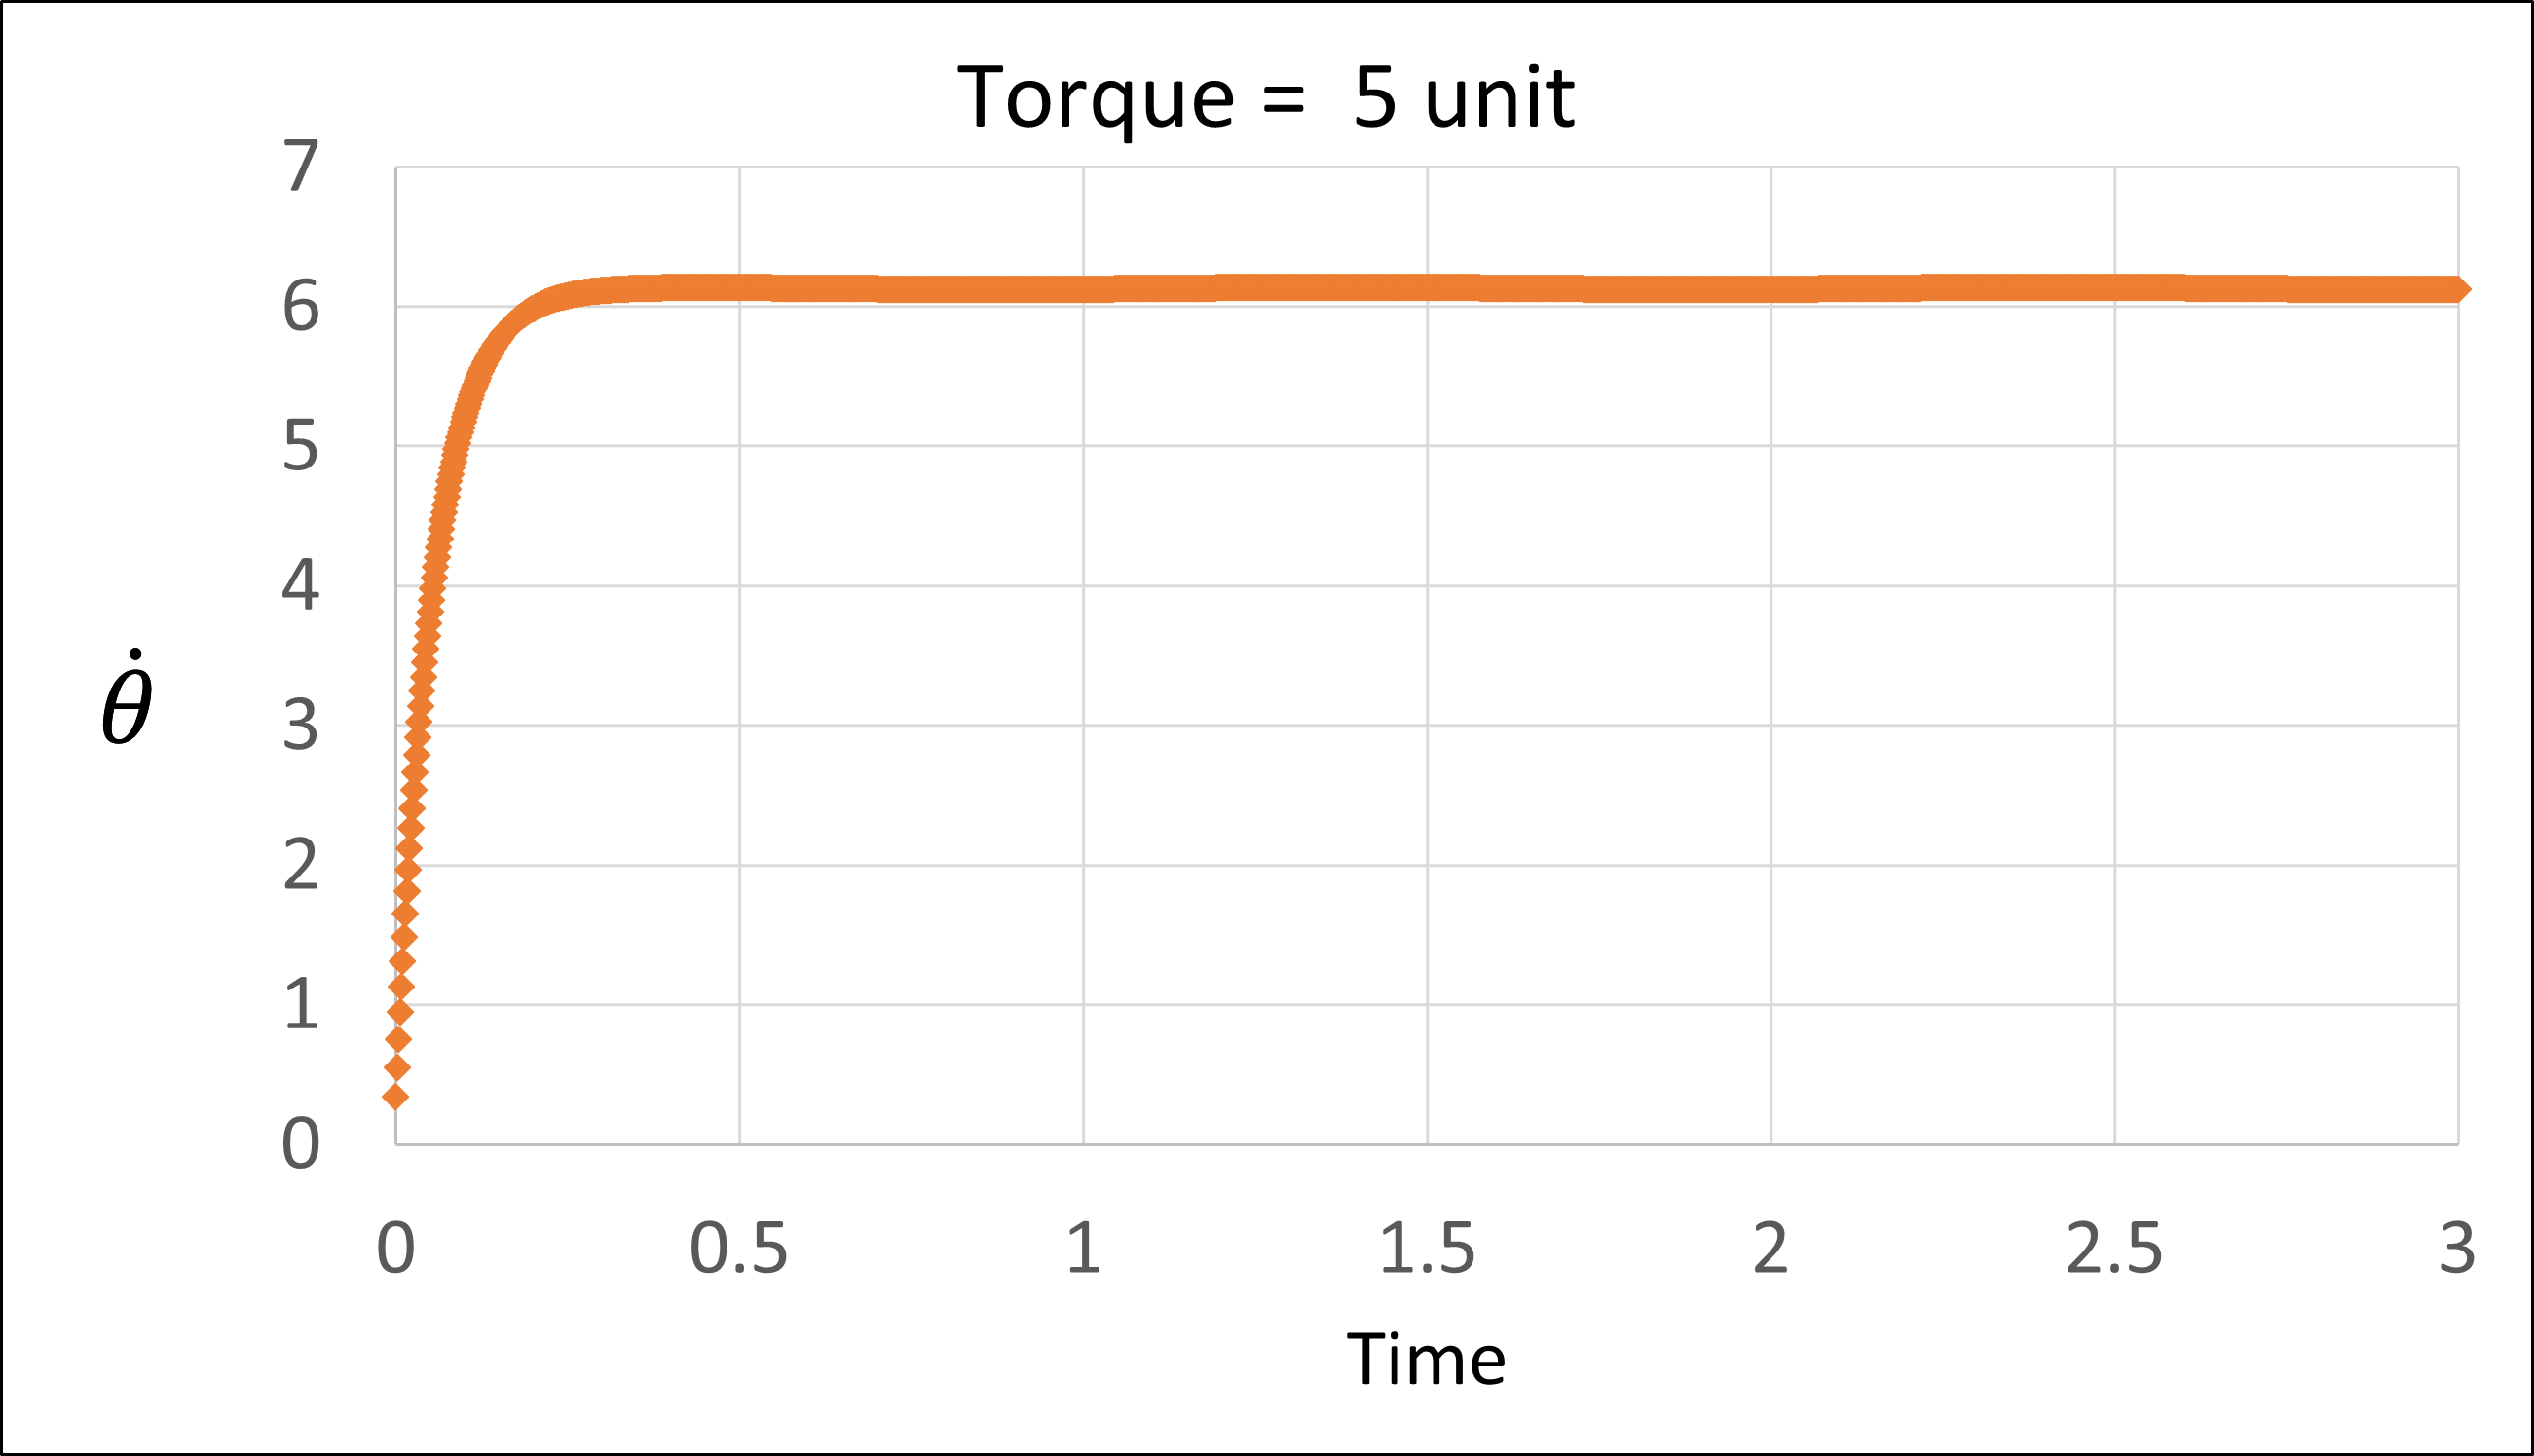
\includegraphics[scale=.4]{Picture5.png}}
	
	\caption{$\dot{\theta}$ for different values of constant torques}
	\label{fig2}
\end{figure}

Now, knowing that $B$ and $G(\Theta)$, compensate for it and get $\ddot{\theta} = 0$. Applying constant torque, gravity compensation and friction to achieve constant acceleration. 

\begin{equation}
	\tau +G(\theta) + B \dot{\theta}=I \ddot{\theta}+B \dot{\theta}+G(\theta)
\end{equation}
System will eventually reach constant acceleration, 
\begin{equation}
	\tau=I \dddot{\theta} \quad \Rightarrow \quad I=\frac{\tau}{\ddot{\theta}}
\end{equation}

Three experiments are performed while applying different constant torques of $(1, 2, 5)$ units. For each constant torque, $\dot{\theta}$ values is collected and imported to excel sheet (which are attached in the zip file), where $\ddot{\theta}$ is calculated using the $500 \; Hz$ frequency given, i.e. 
\begin{equation}
	\ddot{\theta} = \frac{\Delta \dot{\theta}}{\Delta t}
\end{equation}

 Following is the code snippet for this case, where $I$ turns out to be equal to \framebox[1.1\width]{$\mathbf{0.046205}$}, which is taken as the average of three values from Table \ref{table:1}.
 

	
\begin{lstlisting}[style=CStyle]
	#include <stdio.h>
	#include <math.h>
	#include <stdlib.h>
	#ifndef M_PI
	#define M_PI 3.1415927
	#endif
	
	int UTA_ID = 1001937580;
	
	
	double PD_control(theta, theta_dot, theta_ref, theta_dot_ref)
	double theta, theta_dot, theta_ref, theta_dot_ref;
	{
		
		double tau = 1; // tau = 2; // tau = 5;
		//double B = 0.815009;
		//double B = tau/theta_dot;
		//printf("%f\n", theta_dot); //B = 0.815009;
		//double I = 0.046205
		printf("%f %f\n", theta, theta_dot);
		return (tau + b*theta_dot + 2.205195*cos(theta));
	}
\end{lstlisting}	

	\begin{table}[h!]
		\centering
		\begin{tabular}{|c|c|} 
			\hline
			\textbf{Torque value} & \textbf{Inertia value, $I$} \Tstrut \Bstrut\\ [0.5ex] 
			\hline\hline
			$1$ unit & 0.045891\Tstrut\Tstrut \\ \hline
			$2$ unit & 0.046107\Tstrut\Tstrut\Bstrut \\ \hline
			$5$ unit & 0.046617\Tstrut\Tstrut \\[0.5ex] 
			\hline
		\end{tabular}
		\caption{Average of $\ddot{\theta}$ over a time period of $2 \; secs$}
		\label{table:1}
	\end{table}
\newpage
\section{PD Controller Implementation}
With the system parameters identified in Section 1, PD control is implement in this section with gain $K_p$ andd $K_d$. The control force will be equal to, 

\begin{equation}
	F_c = I \; [(K_p (\theta_{ref} - \theta) + K_d (\dot{\theta}_{ref} - \dot{\theta})] + B\dot{\theta} + G(\theta)
\end{equation}

 Fig. (\ref{fig3}) shows the actual implemenation of PD control for two cases. 
\begin{itemize}
	\item Case (a): Initial $\theta_{0} = 0$ and the reference is set as $\theta_{ref} = 1.57$. It could be seen that the PD controller successfully takes the robot manipulator to the set reference value.
	\item Case (b): Here, the initial $\theta_{0} = 1.57$ and the reference is set to $\theta_{ref} = 2.3$. We can see that it reaches the reference value by using the PD control. 
\end{itemize}

\begin{figure}[h]
	
	\begin{minipage}{.5\linewidth}
		\centering
		\subfloat[]{\label{main:a2}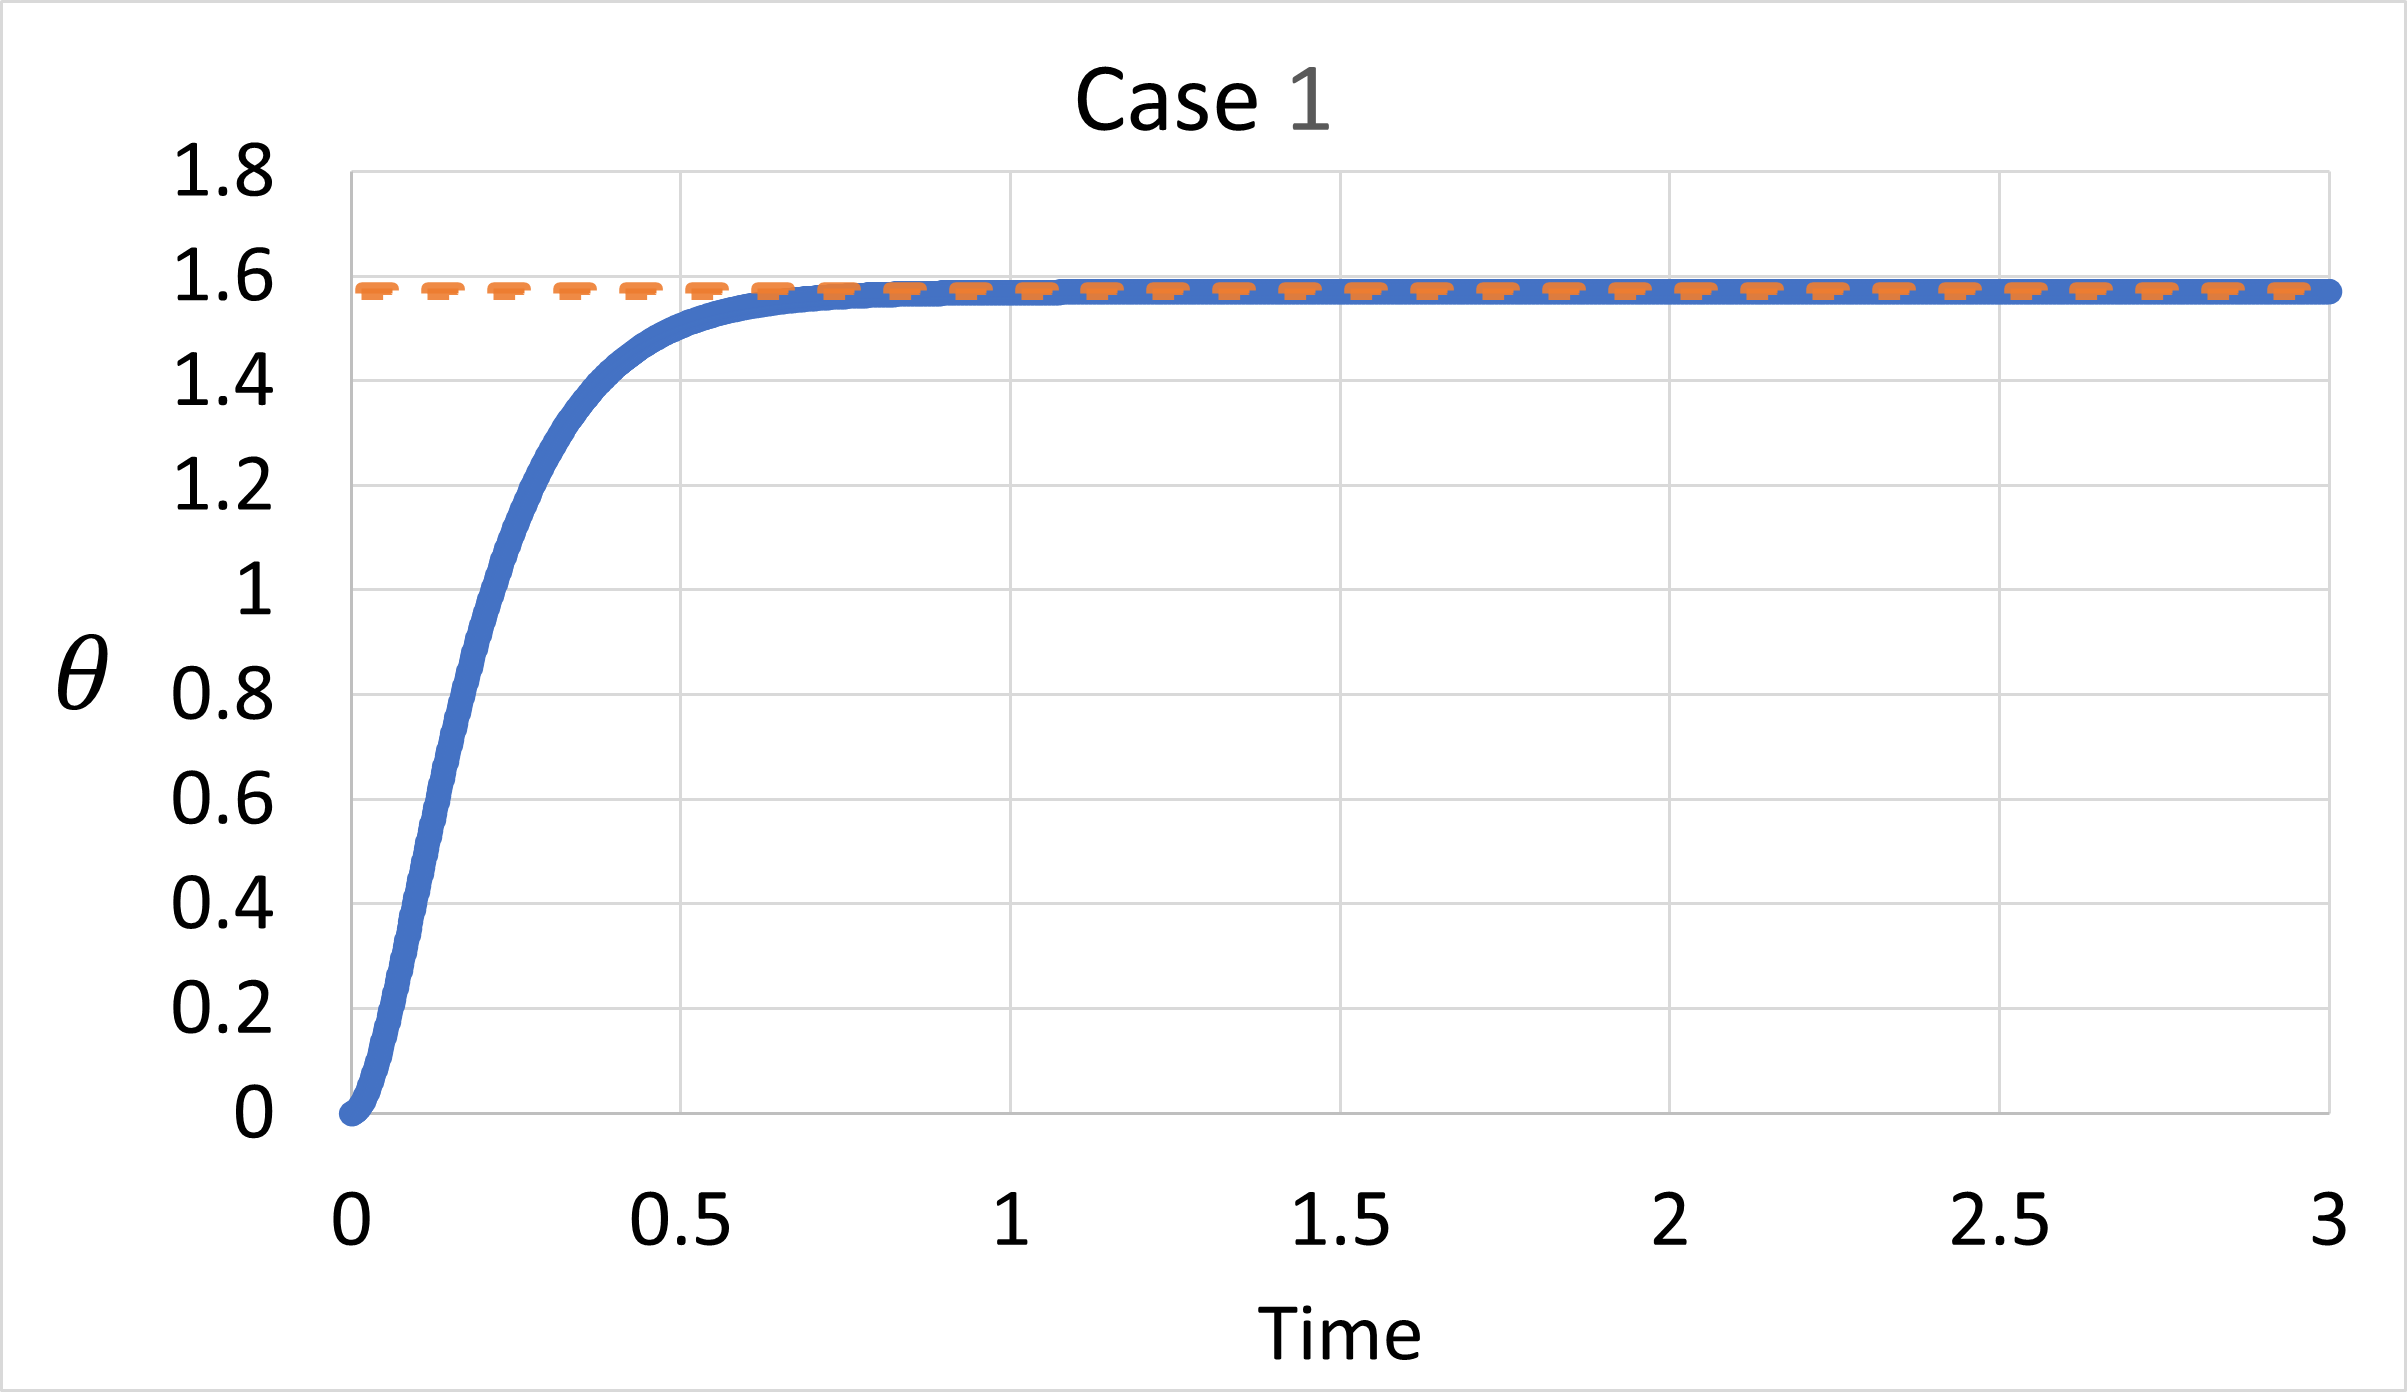
\includegraphics[scale=.4]{pd1.png}}
	\end{minipage}%
	\begin{minipage}{.5\linewidth}
		\centering
		\subfloat[]{\label{main:a3}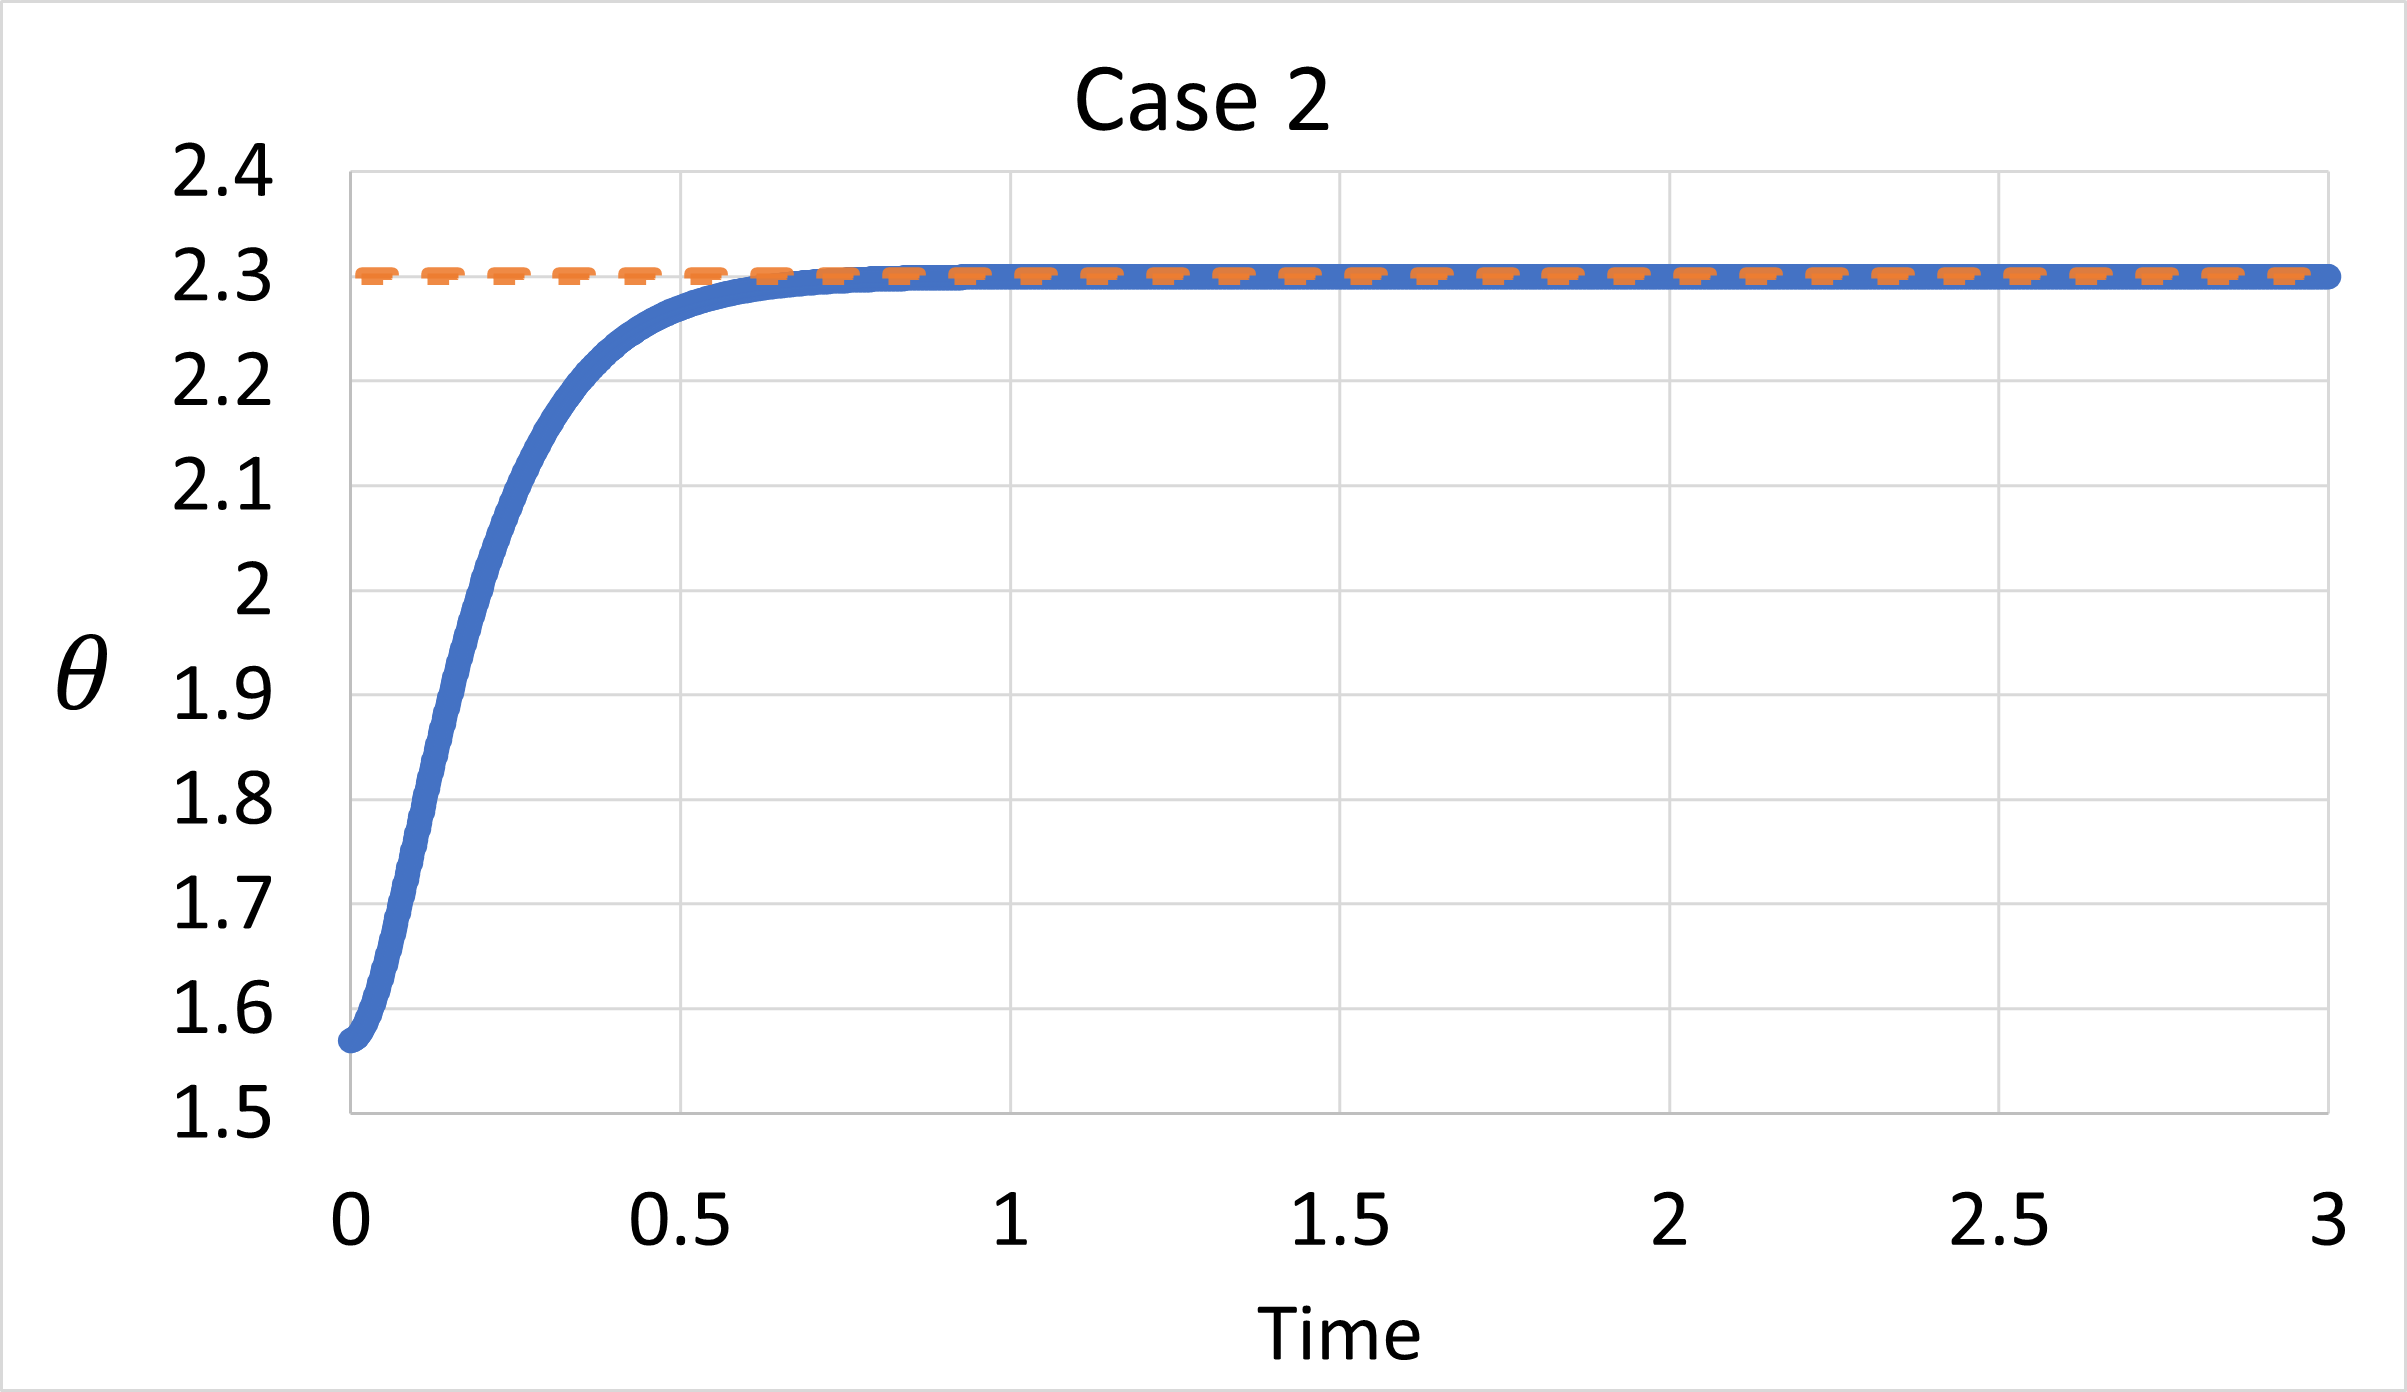
\includegraphics[scale=.4]{pd2.png}}
	\end{minipage}\par\medskip
	
	\caption{${\theta}$ for different intial conditions}
	\label{fig3}
\end{figure}

The overall code that implements the PD control is shown below. 
	
\begin{lstlisting}[style=CStyle]
#include <stdio.h>
#include <math.h>
#include <stdlib.h>
#ifndef M_PI
#define M_PI 3.1415927
#endif

int UTA_ID = 1001937580;


double PD_control(theta, theta_dot, theta_ref, theta_dot_ref)
double theta, theta_dot, theta_ref, theta_dot_ref;
{
	
	double b = 0.815009;
	double I = 0.046205;
	//double b = tau/theta_dot;
	
	printf("%f %f\n", theta, theta_dot);
	double K_p = 100.0;
	double K_d = 2*sqrt(K_p);
	
	double control_force = I*(K_p*(theta_ref-theta) + K_d*(theta_dot_ref-theta_dot)) + b*theta_dot + 2.205195*cos(theta);
	return control_force;
}


\end{lstlisting}	

\end{document}

